%%%%%%%%%%%%%%%%%%%%%%%%%%%%%%%%%%%%%%%%%%%%%%%%%%%%%%%%%%%%%%%%%%%%%%%%
% Escuela Politécnica Superior de la Universidad de Alicante
% Realizado por: Jose Manuel Requena Plens
% Contacto: info@jmrplens.com / Telegram:@jmrplens
%%%%%%%%%%%%%%%%%%%%%%%%%%%%%%%%%%%%%%%%%%%%%%%%%%%%%%%%%%%%%%%%%%%%%%%%

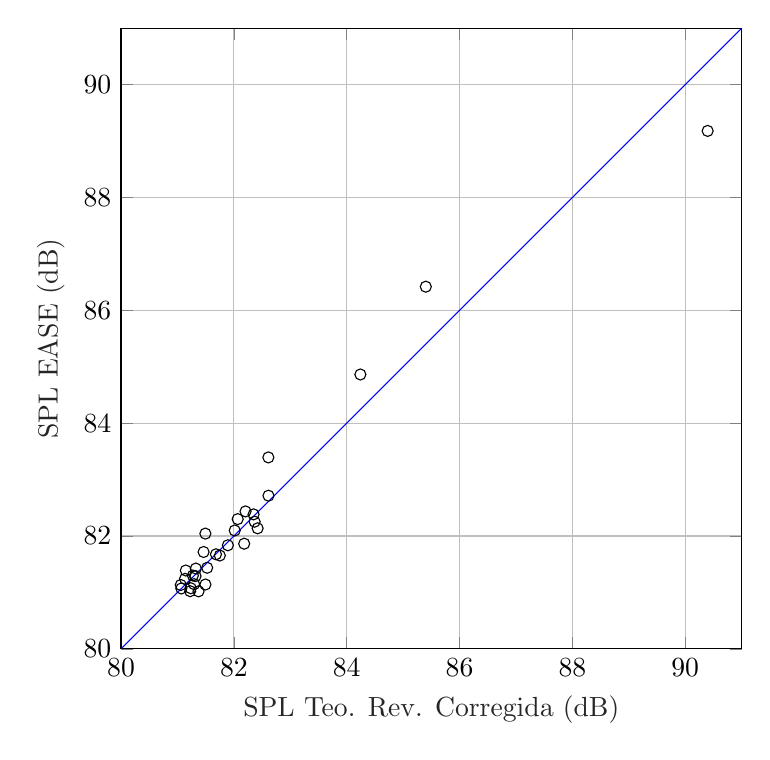
\begin{tikzpicture}

\begin{axis}[%
width=\textwidth,
height=0.65\textwidth,
at={(0\textwidth,0\textwidth)},
scale only axis,
xmin=80,
xmax=91,
xlabel style={font=\color{white!15!black}},
xlabel={SPL Teo. Rev. Corregida (dB)},
ymin=80,
ymax=91,
axis equal image=true,
%minor x tick num= 1,
%minor y tick num= 1,
%ytick distance=0.1,
ylabel style={font=\color{white!15!black}},
ylabel={SPL EASE (dB)},
axis background/.style={fill=white},
xmajorgrids,
xminorgrids,
ymajorgrids,
yminorgrids,
legend style={legend cell align=left, align=left, draw=white!15!black}
]
\addplot [color=black, only marks, mark=o]
  table[row sep=crcr]{%
81.2251663600713	81.0212548219412\\
81.2363689965190	81.0736050871480\\
81.0587718340490	81.1314970364455\\
81.1487112320415	81.3878884354296\\
81.4951924998070	82.0418721632743\\
82.6116352718178	83.3925065130753\\
85.4021853316195	86.4185413027313\\
90.3982646553281	89.1798623386156\\
84.2425825118207	84.8623591998775\\
82.6135122913565	82.7135192859782\\
81.4634891242453	81.7163483969128\\
81.2952042735866	81.1459468769449\\
81.1341656558285	81.2395590249765\\
81.3736867303669	81.0185445830282\\
81.4959826351208	81.1398458110089\\
81.3263223641795	81.4221500117570\\
81.8939660289482	81.8351416684858\\
82.3683576537562	82.2530990929903\\
82.3492400917929	82.3829975408328\\
82.0154843359460	82.0972979971276\\
81.7509835368211	81.6536080542705\\
81.3211075371412	81.2885977800949\\
81.5268252555827	81.4361371317702\\
81.0686463752940	81.0694174464935\\
82.1830625473700	81.8630490038672\\
82.0680524605599	82.2990180096669\\
82.2069902990955	82.4354519254083\\
82.4214071828821	82.1359870202855\\
81.6830817762083	81.6749740343141\\
81.2735704456450	81.2987418474784\\
};

\addplot [blue,samples at={80,91}] {x};
\end{axis}
\end{tikzpicture}%